\section{Proposta}


Este trabalho ataca o problema da detecção de \textit{fake news} binário na língua portuguesa Utilizando a rede Neural BERT. Esta seçâo visa contextualizar alguns tópicos como, por exemplo: Definiçâo do problema; Qual é a base de dados utilizada; Qual o modelo proposto.

% Aqui entram a descrição detalhada do problema sendo tratado e o plano de Solução.

% Aqui será explicada a sua proposta, com cuidado para atingir o objetivo descrito na introdução (ele pode ser lembrado) e como é diferente dos trabalhos correlatos.




\subsection{Definição do problema}

Dado um artigo de notícia $n$, a tarefa de detecção de notícias falsas é prever se essa notícia $n$ é falsa ou verdadeira, isto é,

\begin{center}
    $F(n) =$
    \left\{
    	\begin{array}{ll}
    		0  & \mbox{se } \textit{n é uma notícia falsa} \\
    		1 & \textit{Caso contrário}
    	\end{array}
   
\end{center}

onde $F$ é a função de previsão que queremos aprender.

\subsection{Dataset}

A base de dados utilizada por este trabalho é a \textit{The Fake Br. Corpus}  que foi desenvolvida por \citet{Silva2020}. Esse \textit{dataset} possui um total de 7200 notícias, onde metade dessas notícias é falsa e a outra metade é verdadeira. 

Essa base de dados possui notícias dos seguintes tópicos: economia, ciência e tecnologia, sociedade e notícias diárias, política, religião e, por fim, TV e celebridades. Contudo, vale ressaltar que os tópicos de política, TV e celebridades e sociedade e notícias diárias constituem a maior parte dos dados. A Figura \ref{fig:news_topic_dataset} apresenta como essas notícias se dispersam em cada um desses tópicos. 


\begin{figure}[h]
    \centering
    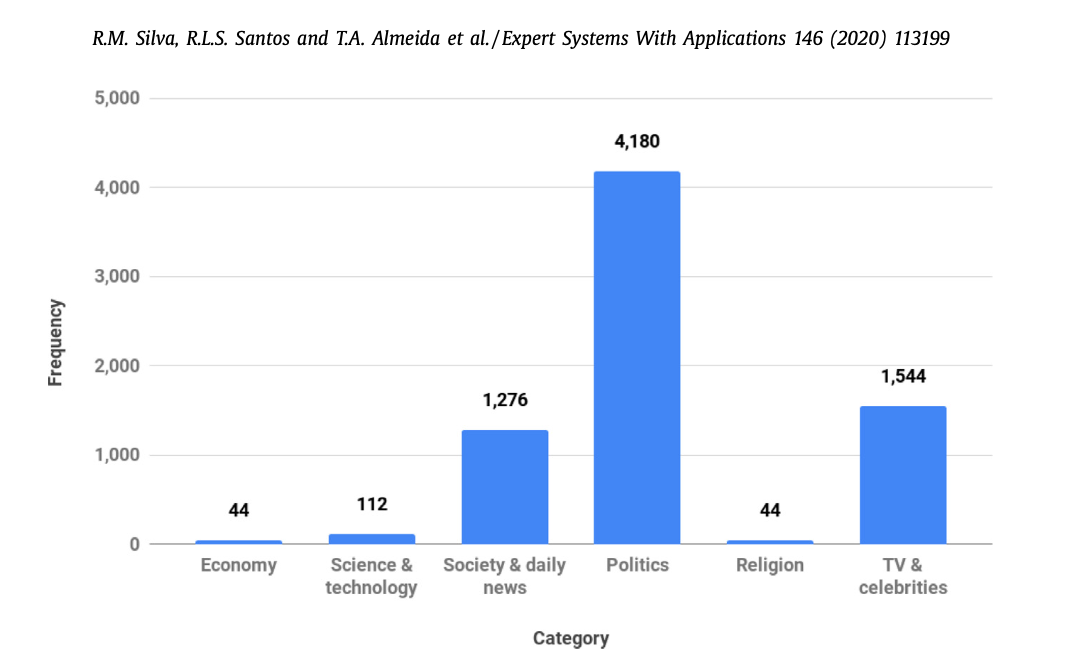
\includegraphics[width=0.85\textwidth]{Imagens/categorias_dataset.png}
    \caption{Frequência das notícias por tópico no Fake Br. Corpus}
    \label{fig:news_topic_dataset}
\end{figure}



\subsection{Modelo Proposto}

O modelo proposto faz uso do \textbf{BERT} (Bidirectional Encoder Representations from Transformers) que é uma técnica para processamento de linguagem natural baseada em \textit{Transformers} que foi desenvolvida pela \textit{Google}. Neste trabalho foi utilizado o Bertimbau (\cite{souza2020bertimbau}) que é um modelo pré-treinado do BERT para o portugês brasileiro. Para este trabalho foi escolhido o Modelo Bertimbau-Base que consiste de 12 camadas de \textit{Transformer encoder}, 12 \textit{attention heads}, 768 \textit{hidden size}, e 110M de parâmetros.\\

O modelo proposto foi construido da seguinte maneira: \\
\begin{enumerate}
    \item Primeiramente, devemos processar o texto de modo a transforma-lo em tokens que deveremos enviar para o classificador;
    \item  Então, extraímos o vetor de \textit{embedding}, de tamanho 768, do token [CLS] provido pelo BERT. (Esse token representa o significado da frase);
    \item A seguir, o utilizamos como \textit{input} para uma camada linear com a função de ativação ReLU;
    \item Por fim temos um vetor de tamanho 2, cada posição desse vetor corresponde a uma categoria dos \textit{labels} (falsa, verdadeira).\\
\end{enumerate}


Toda a implementação do modelo foi realizada em python utilizando a biblioteca pytorch e para o loop de treinamento do modelo foram utilizados o otimizador \textit{Adam} do pytorch com \textit{learning rate} de $1e-5$ e o critério \textit{CrossEntropyLoss} também do pytorch utilizando os parâmetros padrões.

% For a text classification task, we focus our attention on the embedding vector output from the special [CLS] token. This means that we’re going to use the embedding vector of size 768 from [CLS] token as an input for our classifier, which then will output a vector of size the number of classes in our classification task.

% The second variable, which we named pooled_output, contains the embedding vector of [CLS] token. For a text classification task, it is enough to use this embedding as an input for our classifier.

% We then pass the pooled_output variable into a linear layer with ReLU activation function. At the end of the linear layer, we have a vector of size 5, each corresponds to a category of our labels (sport, business, politics, entertainment, and tech).